\section{中間ポジション(1/2)}

\begin{center}
\begin{tabular}{|lcl|}
\hline
この章の基礎練習 & : & 1. 開放弦の練習 2. 「\ref{5th_scale}」の音階練習 3. ベートーヴェン\\
この章の修了課題 & : & 1. 「\ref{2nd-3rd_scale}」の音階練習を正しい音程で暗譜して演奏できる\\
               &   & 2. 「どろぼうかささぎ」を正しい音程で暗譜して演奏できる\\
               &   & 3. モーツァルトを正しい音程で暗譜して演奏できる\\
\hline
\end{tabular}
\end{center}

\begin{flushleft}
\begin{minipage}{300pt}
\subsection{中間ポジションと既出ポジションとの位置関係}
\ \ \ \ この節で勉強する2つのポジションと既出の各ポジションとの関係を
図\addtocounter{figure}{1}\thefigure に示しました。第III・第IVの中間ポジショ
ンのD、A、E線で取れる音は、細い方の隣の弦のハーフ・ポジションに対応し
ています。
\subsection{第II・第IIIの中間ポジションで取れる音}
\begin{music}
\nostartrule
\parindent 0pt
\setclef1{\bass}  
\startpiece
\notes\enotes
\Notes\zchar{16}{G線}\zchar{11}{\bf 1}\wh{b}\zchar{12}{\bf 2}\wh{c}\zchar{13}{\bf 4}\wh{^c}\enotes
\doublebar
\Notes\zchar{11}{\bf 1}\wh{b}\zchar{12}{\bf 2}\wh{c}\zchar{13}{\bf 4}\wh{_d}\enotes
\doublebar
\Notes\zchar{16}{D線}\zchar{9}{\bf 1}\wh{'^F}\zchar{9}{\bf 2}\wh{G}\zchar{9}{\bf 4}\wh{^G}\enotes
\doublebar
\Notes\zchar{10}{\bf 1}\wh{'_G}\zchar{10}{\bf 2}\wh{=G}\zchar{10}{\bf 4}\wh{!_a}\enotes
\setdoublebar
\endpiece
\startpiece
\notes\enotes
\Notes\zchar{14}{A線}\zchar{9}{\bf 1}\wh{'^C}\zchar{9}{\bf 2}\wh{D}\zchar{9}{\bf 4}\wh{^D}\enotes
\doublebar
\Notes\zchar{9}{\bf 1}\wh{'_D}\zchar{9}{\bf 2}\wh{=D}\zchar{9}{\bf 4}\wh{_E}\enotes
\doublebar
\Notes\zchar{14}{E線}\zchar{9}{\bf 1}\wh{^G}\zchar{9}{\bf 2}\wh{'A}\zchar{9}{\bf 4}\wh{^A}\enotes
\doublebar
\Notes\zchar{9}{\bf 1}\wh{'_A}\zchar{9}{\bf 2}\wh{=A}\zchar{9}{\bf 4}\wh{_B}\enotes
\setdoublebar
\endpiece
\end{music}
\end{minipage}
\hfill
\begin{minipage}{100pt}
\begin{center}
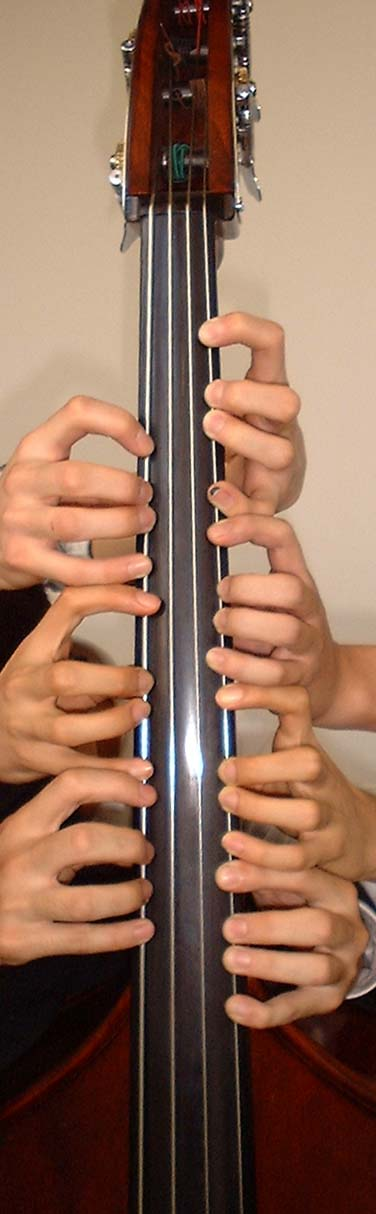
\includegraphics[height=7.5cm]{../Vol1/Pics/Position/1st-4th.epsi}\\
{\flushleft\small 図\thefigure : 中間ポジション\\}
\end{center}
\end{minipage}
\end{flushleft}

\subsection{音階練習 \label{2nd-3rd_scale}}
\begin{music}
\nostartrule
\parindent 0pt
\setclef1{\bass}  
\generalsignature{4}    
\startpiece
\notes\zchar{14}{ホ長調(E-dur)音階}\enotes
\Notes\qu{E}\enotes
\notes\ibu{0}{F}{3}\islurd{0}{F}\zchar{-6}{I}\zchar{8}{\bf 1}\qb{0}{F}\tbu{0}\tslur{0}{G}\qb{0}{G}\enotes
\notes\ibl{0}{'A}{3}\qb{0}{A}\qb{0}{B}\qb{0}{C}\tbl{0}\zchar{-4}{half}\zchar{8}{\bf 1}\qb{0}{D}\enotes
\bar
\Notes\zchar{-4}{I}\zchar{8}{\bf 1}\ql{'E}\enotes
\notes\ibl{0}{'F}{3}\isluru{0}{F}\qb{0}{F}\tbl{0}\tslur{0}{G}\loffset{0.2}{\zchar{-4}{half}}\zchar{10}{\bf 1}\qb{0}{G}\enotes
\notes\ibl{0}{a}{3}\qb{0}{a}\loffset{0.7}{\zchar{-5}{\small [}}\roffset{0.3}{\zchar{-4}{\small II}}\zchar{-7}{\small III}\zchar{11}{\bf 1}\qb{0}{b}\qb{0}{c}\tbl{0}\zchar{-4}{IV}\zchar{14}{\bf 2}\qb{0}{d}\enotes
\bar
\Notes\ql{e}\enotes
\notes\ibl{0}{d}{-2}\isluru{0}{d}\qb{0}{d}\tbl{0}\tslur{0}{c}\loffset{0.7}{\zchar{-5}{\small [}}\roffset{0.3}{\zchar{-4}{\small II}}\zchar{-7}{\small III}\zchar{14}{\bf 4}\qb{0}{c}\enotes
\notes\ibl{0}{b}{-3}\qb{0}{b}\zchar{-4}{half}\zchar{10}{\bf 2}\qb{0}{a}\qb{0}{'G}\tbl{0}\zchar{-4}{I}\zchar{8}{\bf 4}\qb{0}{F}\enotes
\bar
\notes\ibl{0}{'E}{-3}\qb{0}{E}\loffset{1.25}{\zchar{-7}{half}}\zchar{8}{\bf 1}\qb{0}{D}\zchar{-7}{I}\zchar{8}{\bf 4}\qb{0}{C}\tbl{0}\qb{0}{B}\enotes
\notes\ibu{0}{'A}{-3}\qb{0}{A}\qb{0}{!G}\qb{0}{F}\tbu{0}\qb{0}{E}\enotes
\endpiece

\generalsignature{1}    
\startpiece
\notes\zchar{14}{ホ短調(e-moll)音階}\enotes
\Notes\qu{E}\enotes
\notes\ibu{0}{F}{3}\islurd{0}{F}\zchar{-6}{I}\zchar{8}{\bf 1}\qb{0}{F}\tbu{0}\tslur{0}{G}\qb{0}{G}\enotes
\notes\ibl{0}{'A}{3}\qb{0}{A}\qb{0}{B}\qb{0}{^C}\tbl{0}\zchar{-4}{half}\zchar{8}{\bf 1}\qb{0}{^D}\enotes
\bar
\Notes\zchar{-4}{I}\zchar{8}{\bf 1}\ql{'E}\enotes
\notes\ibl{0}{'F}{3}\isluru{0}{F}\qb{0}{F}\tbl{0}\tslur{0}{G}\qb{0}{G}\enotes
\notes\ibl{0}{a}{3}\qb{0}{a}\loffset{0.7}{\zchar{-5}{\small [}}\roffset{0.3}{\zchar{-4}{\small II}}\zchar{-7}{\small III}\zchar{12}{\bf 1}\qb{0}{b}\qb{0}{^c}\tbl{0}\zchar{-4}{IV}\zchar{14}{\bf 2}\qb{0}{^d}\enotes
\bar
\Notes\ql{e}\enotes
\notes\ibl{0}{d}{-2}\isluru{0}{d}\qb{0}{=d}\tbl{0}\tslur{0}{c}\zchar{-4}{II}\zchar{14}{\bf 4}\qb{0}{=c}\enotes
\notes\ibl{0}{b}{-3}\qb{0}{b}\zchar{-4}{I}\zchar{12}{\bf 1}\qb{0}{a}\qb{0}{'G}\tbl{0}\qb{0}{F}\enotes
\bar
\notes\ibl{0}{'E}{-3}\qb{0}{E}\qb{0}{D}\qb{0}{C}\tbl{0}\qb{0}{B}\enotes
\notes\ibu{0}{'A}{-3}\qb{0}{A}\qb{0}{!G}\qb{0}{F}\tbu{0}\qb{0}{E}\enotes
\endpiece
\end{music}

\clearpage

\subsection{第II・第IIIの中間ポジションで弾ける名曲}
\documentclass{jarticle}
\usepackage{musixdoc}
\startmuflex\makeindex

\begin{document}

\subsubsection*{���å�����: �η�֤ɤ��ܤ����������׽��ʤ��}
\begin{music}
\nostartrule
\setclef1{\bass}
\generalsignature{1}    
\generalmeter{\meterfrac34}
\parindent 0pt
\startbarno=115
\def\writebarno{\tenrm\the\barno\barnoadd}
\def\raisebarno{2\internote}
\def\shiftbarno{0.1\Interligne}
\systemnumbers
\startpiece\bigaccid
\notes\zchar{18}{\bf (Allegro)}\zchar{-5}{\ff}\enotes
\Notes\zchar{-5}{I}\zchar{11}{\downbow}\zchar{9}{\bf 1}\ql{'E}\qp\enotes
\notes\xtuplet{3}{'G}\ibl{0}{E}{0}\zchar{9}{\upbow}\qb{0}{E}\qb{0}{E}\tbl{0}\qb{0}{E}\enotes
\bar
\Notes\loffset{1.5}{\zchar{-5}{\it marc.}}\zchar{9}{\downbow}\ql{'E}\loffset{0.6}{\zchar{-5}{\small [}}\roffset{0.3}{\zchar{-4}{\small II}}\zchar{-7}{\small III}\zchar{12}{\upbow}\zchar{9}{\bf 4}\ql{^G}\zchar{14}{\upbow}\zchar{11}{\bf 1}\ql{!b}\enotes
\bar
\Notes\zchar{-4}{IV}\zchar{-8}{\ppfftwenty sf}\isluru{0}{e}\zchar{16}{\downbow}\zchar{14}{\bf 4}\ql{e}\enotes
\notes\ibl{0}{e}{-3}\tslur{0}{e}\qb{0}{e}\upz{d}\qb{0}{^d}\loffset{0.7}{\zchar{-5}{\small [}}\roffset{0.3}{\zchar{-4}{\small II}}\zchar{-7}{\small III}\zchar{13}{\bf 4}\upz{c}\qb{0}{^c}\tbl{0}\zchar{12}{\bf 1}\upz{b}\qb{0}{b}\enotes
\bar
\notes\ibl{0}{a}{-4}\loffset{1}{\zchar{-4}{half}}\zchar{11}{\bf 2}\upz{a}\qb{0}{a}\upz{'G}\qb{0}{^G}\zchar{-5}{I}\zchar{10}{\bf 4}\upz{F}\qb{0}{F}\upz{E}\qb{0}{E}\loffset{0.7}{\zchar{-8}{\small [}}\roffset{0.3}{\zchar{-7}{\small II}}\zchar{-10}{\small III}\zchar{9}{\bf 4}\upz{D}\qb{0}{^D}\tbl{0}\zchar{9}{\bf 1}\upz{C}\qb{0}{^C}\enotes
\bar
\Notes\zchar{-4}{I}\zchar{9}{\bf 1}\qu{'B}\qp\enotes
\notes\xtuplet{3}{!c}\ibu{0}{'B}{0}\qb{0}{B}\qb{0}{B}\tbu{0}\qb{0}{B}\enotes
\bar
\Notes\zchar{-4}{\icresc}\qu{'B}\loffset{0.7}{\zchar{-9}{\small [}}\roffset{0.3}{\zchar{-8}{\small II}}\zchar{-11}{\small III}\zchar{8}{\bf 4}\ql{^D}\zchar{10}{\bf 1}\ql{F}\zchar{-4}{\tcresc}\enotes
\bar
\Notes\zchar{-4}{\ppfftwenty sf}\isluru{0}{b}\ql{b}\enotes
\notes\ibl{0}{b}{-1}\tslur{0}{b}\qb{0}{b}\upz{c}\qb{0}{^c}\upz{b}\qb{0}{b}\tbl{0}\zchar{-4}{half}\zchar{11}{\bf 2}\upz{a}\qb{0}{a}\enotes
\bar
\notes\ibl{0}{'G}{-4}\upz{G}\qb{0}{^G}\zchar{-5}{I}\zchar{10}{\bf 4}\upz{F}\qb{0}{F}\upz{E}\qb{0}{E}\loffset{0.7}{\zchar{-7}{\small [}}\roffset{0.3}{\zchar{-6}{\small II}}\zchar{-9}{\small III}\zchar{9}{\bf 4}\upz{D}\qb{0}{^D}\zchar{9}{\bf 1}\upz{C}\qb{0}{^C}\tbl{0}\zchar{-8}{I}\zchar{9}{\bf 1}\upz{B}\qb{0}{B}\enotes
\bar
\Notes\ql{'E}\qp\enotes
\notes\xtuplet{3}{'G}\ibl{0}{E}{0}\qb{0}{E}\qb{0}{E}\tbl{0}\qb{0}{E}\enotes
\bar
\Notes\zchar{-4}{\icresc}\ql{'E}\zchar{-3}{II}\zchar{9}{\bf 4}\ql{=G}\ql{!b}\zchar{-4}{\tcresc}\enotes
\bar
\Notes\zchar{-4}{IV}\zchar{-7}{\ppfftwenty sf}\isluru{0}{e}\zchar{14}{\bf 4}\ql{e}\enotes
\notes\ibl{0}{e}{-3}\tslur{0}{e}\qb{0}{e}\upz{d}\qb{0}{=d}\zchar{-4}{II}\zchar{13}{\bf 4}\upz{c}\qb{0}{=c}\tbl{0}\upz{b}\qb{0}{b}\enotes
\bar
\notes\ibl{0}{a}{-2}\zchar{-4}{III}\zchar{11}{\bf 4}\upz{a}\qb{0}{a}\upz{'G}\qb{0}{=G}\upz{!a}\qb{0}{a}\upz{'G}\qb{0}{G}\zchar{-5}{I}\zchar{10}{\bf 4}\upz{F}\qb{0}{F}\tbl{0}\upz{E}\qb{0}{E}\enotes
\bar
\Notes\zchar{-6}{II}\zchar{9}{\bf 4}\ql{'=D}\qp\enotes
\notes\xtuplet{3}{'F}\ibl{0}{D}{0}\qb{0}{D}\qb{0}{D}\tbl{0}\qb{0}{D}\enotes
\bar
\Notes\zchar{-6}{\icresc}\ql{'D}\ql{F}\zchar{-4}{IV}\zchar{10}{\bf 1}\ql{!a}\zchar{-6}{\tcresc}\enotes
\bar
\Notes\zchar{-4}{\ppfftwenty sf}\isluru{0}{d}\ql{d}\enotes
\notes\ibl{0}{d}{-1}\tslur{0}{d}\qb{0}{d}\upz{e}\qb{0}{e}\upz{d}\qb{0}{d}\tbl{0}\loffset{0.7}{\zchar{-5}{\small [}}\roffset{0.3}{\zchar{-4}{\small II}}\zchar{-7}{\small III}\zchar{13}{\bf 4}\upz{c}\qb{0}{c}\enotes
\bar
\notes\ibl{0}{b}{-4}\upz{b}\qb{0}{b}\zchar{-4}{III}\zchar{11}{\bf 4}\upz{a}\qb{0}{a}\upz{'G}\qb{0}{G}\zchar{-5}{I}\zchar{10}{\bf 4}\upz{F}\qb{0}{F}\upz{E}\qb{0}{E}\tbl{0}\zchar{-6}{II}\zchar{9}{\bf 4}\upz{D}\qb{0}{D}\enotes
\bar
\Notes\ql{'G}\qp\qp\enotes
\setdoublebar\endpiece
\end{music}

\endmuflex
\end{document}

\documentclass{jarticle}
\usepackage{musixdoc}
\startmuflex\makeindex

\begin{document}
\subsubsection*{�֥�å��ʡ�: �������8�� ��ûĴ ��4�ھϤ��}

\begin{music}
\nostartrule
\setclef1{\bass}
\generalsignature{-3}    
\generalmeter{\allabreve}
\parindent 0pt
\startbarno=135
\def\writebarno{\tenrm\the\barno\barnoadd}
\def\raisebarno{2\internote}
\def\shiftbarno{0.1\Interligne}
\systemnumbers
\startpiece\bigaccid
\notes\zchar{17}{\LARGE \bf I}\zchar{21}{\hspace{1em} nicht gebunden (Feierlich, nicht schnell (\metron{\hu}{69}) $\rightarrow$ Langsamer (\metron{\hu}{60})}\zchar{17}{\hspace{8em} $\rightarrow$ noch langsamer $\rightarrow$ a tempo $\rightarrow$)}\enotes
\Notes\zchar{-4}{\p}\zchar{12}{\downbow}\zchar{9}{\bf 4}\ql{'E}\zchar{12}{\upbow}\zchar{9}{\bf 4}\qu{B}\ql{E}\qu{B}\enotes
\bar
\Notes\ql{'E}\zchar{9}{\bf 1}\qu{A}\ql{E}\enotes
\notes\ibl{0}{'D}{1}\zchar{12}{\upbow}\zchar{9}{\bf 2}\ust{D}\qb{0}{D}\tbl{0}\zchar{12}{\downbow}\zchar{9}{\bf 4}\ust{E}\qb{0}{E}\enotes
\bar
\Notes\zchar{12}{\upbow}\zchar{9}{\bf 4}\ql{'F}\enotes
\notes\ibl{0}{'E}{1}\zchar{12}{\downbow}\zchar{9}{\bf 1}\ust{E}\qb{0}{E}\tbl{0}\zchar{12}{\upbow}\zchar{9}{\bf 2}\ust{F}\qb{0}{F}\enotes
\Notes\zchar{12}{\downbow}\zchar{9}{\bf 4}\ql{'_G}\enotes
\notes\ibl{0}{'F}{-1}\zchar{12}{\upbow}\zchar{9}{\bf 4}\ust{F}\qb{0}{F}\tbl{0}\zchar{12}{\downbow}\zchar{9}{\bf 1}\ust{E}\qb{0}{E}\enotes
\bar
\Notes\zchar{9}{\upbow}\ql{'F}\enotes
\notes\ibl{0}{'G}{1}\zchar{13}{\downbow}\zchar{10}{\bf 1}\ust{G}\qb{0}{_G}\tbl{0}\zchar{14}{\upbow}\zchar{11}{\bf 4}\ust{!a}\qb{0}{a}\enotes
\Notes\zchar{14}{\downbow}\zchar{11}{\bf 4}\ql{b}\zchar{10}{\upbow}\qu{'B}\enotes
\bar
\Notes\zchar{-6}{\mf}\zchar{10}{\downbow}\lst{'C}\qu{_C}\enotes
\notes\ibu{0}{G}{2}\zchar{12}{\upbow}\zchar{9}{\bf 1}\lst{G}\islurd{0}{F}\qb{0}{_G}\tbu{0}\lst{'A}\tslur{0}{!G}\qb{0}{'A}\enotes
\Notes\zchar{12}{\downbow}\zchar{9}{\bf 1}\lst{'B}\qu{B}\enotes
\notes\zchar{8}{\upbow}\ibu{0}{F}{2}\lst{F}\islurd{0}{E}\qb{0}{F}\tbu{0}\zchar{9}{\bf 1}\lst{G}\tslur{0}{F}\qb{0}{G}\enotes
\bar
\Notes\zchar{9}{\downbow}\lst{'A}\qu{A}\enotes
\notes\zchar{12}{\upbow}\zchar{9}{\bf 2}\ibu{0}{G}{-2}\lst{G}\islurd{0}{F}\qb{0}{_G}\tbu{0}\lst{F}\tslur{0}{E}\qb{0}{F}\enotes
\Notes\zchar{9}{\downbow}\lst{G}\qu{G}\enotes
\Notes\zchar{9}{\upbow}\ust{'E}\ql{E}\enotes
\bar
\Notes\zchar{12}{\downbow}\zchar{9}{\bf 1}\ust{'G}\ql{_G}\enotes
\notes\ibl{0}{'D}{1}\zchar{9}{\upbow}\ust{D}\isluru{0}{F}\qb{0}{_D}\tbl{0}\ust{E}\tslur{0}{F}\qb{0}{E}\enotes
\Notes\zchar{12}{\downbow}\zchar{9}{\bf 2}\ust{'F}\ql{F}\enotes
\notes\ibu{0}{'C}{1}\zchar{9}{\upbow}\lst{C}\islurd{0}{B}\qb{0}{C}\tbu{0}\lst{D}\tslur{0}{B}\qb{0}{D}\enotes
\bar
\Notes\zchar{12}{\downbow}\zchar{9}{\bf 4}\ust{'E}\ql{E}\enotes
\notes\ibu{0}{'D}{-1}\zchar{9}{\upbow}\lst{D}\islurd{0}{B}\qb{0}{_D}\tbu{0}\zchar{12}{\bf 2}\lst{C}\tslur{0}{B}\qb{0}{C}\enotes
\Notes\zchar{9}{\downbow}\ust{'D}\ql{D}\enotes
\Notes\zchar{12}{\upbow}\zchar{9}{\bf 4}\lst{'B}\qu{B}\enotes
\bar
\Notes\zchar{-4}{\f}\zchar{15}{\downbow}\zchar{13}{\bf 4}\ql{_d}\enotes
\notes\ibl{0}{a}{1}\zchar{10}{\downbow}\qb{0}{a}\tbl{0}\zchar{15}{\upbow}\zchar{12}{\bf 1}\ust{b}\qb{0}{b}\enotes
\Notes\zchar{13}{\downbow}\ust{c}\ql{c}\enotes
\Notes\zchar{11}{\upbow}\lst{'C}\qu{C}\enotes
\bar
\Notes\zchar{11}{\downbow}\ql{b}\enotes
\notes\ibl{0}{'F}{1}\zchar{9}{\downbow}\qb{0}{F}\tbl{0}\zchar{10}{\upbow}\ust{G}\qb{0}{=G}\enotes
\Notes\zchar{13}{\downbow}\zchar{11}{\bf 4}\ust{a}\ql{a}\enotes
\Notes\zchar{9}{\upbow}\lst{'A}\qu{A}\enotes
\bar
\Notes\zchar{12}{\downbow}\zchar{9}{\bf 1}\ql{'_G}\enotes
\notes\ibl{0}{'D}{1}\zchar{9}{\downbow}\qb{0}{_D}\tbl{0}\zchar{9}{\upbow}\ust{E}\qb{0}{E}\enotes
\Notes\zchar{12}{\downbow}\zchar{9}{\bf 2}\ql{'F}\enotes
\notes\ibu{0}{'C}{1}\zchar{11}{\downbow}\qb{0}{C}\tbu{0}\zchar{12}{\upbow}\lst{D}\qb{0}{D}\enotes
\bar
\Notes\zchar{12}{\downbow}\zchar{9}{\bf 1}\ql{'E}\enotes
\notes\ibu{0}{'B}{1}\zchar{10}{\downbow}\qb{0}{B}\tbu{0}\zchar{13}{\upbow}\zchar{10}{\bf 2}\lst{C}\qb{0}{C}\enotes
\Notes\zchar{8}{\downbow}\ql{'_D}\enotes
\notes\ibu{0}{'A}{1}\zchar{12}{\downbow}\zchar{9}{\bf 1}\qb{0}{A}\tbu{0}\zchar{9}{\upbow}\lst{B}\qb{0}{B}\enotes
\bar
\Notes\zchar{-7}{\it poco a poco dim. - - - - - - - - - - - - - - - - - - -}\islurd{0}{'C}\zchar{12}{\downbow}\zchar{9}{\bf 4}\qu{C}\enotes
\notes\ibu{0}{'B}{-1}\qb{0}{B}\tbu{0}\zchar{9}{\bf 4}\qb{0}{A}\enotes
\Notes\tslur{0}{G}\qu{G}\enotes
\Notes\zchar{11}{\upbow}\zchar{8}{\bf 1}\lst{F}\qu{F}\enotes
\bar
\Notes\islurd{0}{'C}\qu{C}\enotes
\notes\ibu{0}{'B}{-1}\qb{0}{B}\tbu{0}\qb{0}{A}\enotes
\Notes\tslur{0}{G}\qu{G}\enotes
\Notes\lst{F}\qu{F}\enotes
\bar
\Notes\islurd{0}{'C}\qu{C}\enotes
\notes\ibu{0}{'B}{-1}\qb{0}{B}\tbu{0}\qb{0}{A}\enotes
\Notes\tslur{0}{G}\qu{G}\enotes
\Notes\lst{F}\qu{F}\enotes
\bar
\Notes\zchar{-7}{\it - - - - - - - - - -}\islurd{0}{'C}\qu{_C}\enotes
\notes\ibu{0}{'B}{-1}\qb{0}{B}\tbu{0}\qb{0}{A}\enotes
\Notes\tslur{0}{G}\qu{_G}\enotes
\Notes\lst{F}\qu{F}\zchar{16}{\LARGE \bf K}\enotes
\bar
\Notes\zchar{16}{\hspace{1em}nicht gebunden}\zchar{-4}{\p}\zchar{12}{\downbow}\zchar{9}{\bf 4}\ql{'E}\zchar{12}{\upbow}\zchar{9}{\bf 4}\qu{B}\ql{E}\qu{B}\enotes
\bar
\Notes\ql{'E}\qu{A}\ql{E}\enotes
\notes\ibl{0}{'D}{2}\zchar{9}{\upbow}\qb{0}{D}\tbl{0}\zchar{9}{\downbow}\qb{0}{E}\enotes
\bar
\Notes\zchar{12}{\upbow}\zchar{9}{\bf 4}\ql{'F}\enotes
\notes\ibl{0}{'E}{1}\zchar{9}{\downbow}\qb{0}{E}\tbl{0}\zchar{12}{\upbow}\zchar{9}{\bf 2}\qb{0}{F}\enotes
\Notes\zchar{9}{\downbow}\ql{'_G}\enotes
\notes\ibl{0}{'F}{-1}\zchar{12}{\upbow}\zchar{9}{\bf 4}\qb{0}{F}\tbl{0}\zchar{9}{\downbow}\qb{0}{E}\enotes
\bar
\Notes\zchar{9}{\upbow}\ql{'F}\enotes
\notes\ibl{0}{'G}{2}\zchar{12}{\downbow}\zchar{9}{\bf 1}\qb{0}{_G}\tbl{0}\zchar{9}{\upbow}\qb{0}{!a}\enotes
\Notes\zchar{13}{\downbow}\zchar{11}{\bf 4}\ql{b}\zchar{8}{\upbow}\qu{'B}\enotes
\bar
\Notes\zchar{-4}{\f}\zchar{9}{\downbow}\ql{'E}\enotes
\notes\ibu{0}{'B}{1}\zchar{9}{\downbow}\qb{0}{B}\tbu{0}\zchar{13}{\upbow}\zchar{10}{\bf 2}\lst{C}\qb{0}{C}\enotes
\Notes\zchar{9}{\downbow}\ust{'D}\ql{_D}\zchar{9}{\upbow}\ust{D}\ql{D}\enotes
\bar
\Notes\zchar{9}{\downbow}\ql{'_G}\enotes
\notes\ibl{0}{'D}{2}\zchar{9}{\downbow}\qb{0}{_D}\tbl{0}\zchar{12}{\upbow}\zchar{9}{\bf 1}\ust{E}\qb{0}{E}\enotes
\Notes\zchar{9}{\downbow}\ust{'F}\ql{F}\zchar{9}{\upbow}\lst{!F}\qu{F}\enotes
\bar
\Notes\zchar{-4}{\ff}\zchar{13}{\downbow}\zchar{11}{\bf 1}\ql{b}\enotes
\notes\ibl{0}{'F}{1}\zchar{9}{\downbow}\qb{0}{F}\tbl{0}\zchar{10}{\upbow}\ust{G}\qb{0}{=G}\enotes
\Notes\zchar{13}{\downbow}\zchar{11}{\bf 1}\ust{a}\ql{a}\enotes
\notes\ibl{0}{b}{1}\zchar{12}{\upbow}\ust{b}\isluru{0}{c}\qb{0}{b}\tbl{0}\ust{c}\tslur{0}{d}\zchar{14}{\bf 2}\qb{0}{c}\enotes
\bar
\Notes\zchar{12}{\downbow}\ql{_d}\enotes
\notes\ibl{0}{c}{-1}\zchar{12}{\downbow}\qb{0}{c}\tbl{0}\zchar{15}{\upbow}\ust{b}\zchar{12}{\bf 1}\qb{0}{b}\enotes
\Notes\zchar{12}{\downbow}\ust{c}\ql{c}\zchar{9}{\upbow}\lst{'C}\qu{C}\enotes
\mulooseness=0
\setdoublebar
\endpiece
\end{music}
\endmuflex
\end{document}

\subsubsection*{ベートーヴェン: 交響曲第6番 ヘ長調 「田園」 第4楽章より}
\begin{music}
\nostartrule
\setclef1{\bass}
\generalsignature{-4}    
\generalmeter{\meterfrac44}
\parindent 0pt
\startbarno=78
\def\writebarno{\tenrm\the\barno\barnoadd}
\def\raisebarno{2\internote}
\def\shiftbarno{0.1\Interligne}
\systemnumbers
\startpiece\bigaccid
\notes\zchar{20}{\bf \LARGE E}\zchar{16}{\bf (Allegro)}\enotes
\NOtes\zchar{-4}{\ff}\zchar{11}{\downbow}\zchar{-9}{II}\zchar{9}{\bf 4}\hlp{'G}\enotes
\Notes\zchar{-4}{\ppfftwenty sf}\zchar{12}{\upbow}\zchar{-9}{half}\zchar{9}{\bf 4}\isluru{0}{'F}\ql{F}\enotes
\bar
\NOtes\tslur{0}{'E}\hlp{E}\enotes
\Notes\zchar{-4}{\ppfftwenty sf}\zchar{-9}{II}\zchar{9}{\bf 4}\isluru{0}{'D}\ql{=D}\enotes
\bar
\NOtes\tslur{0}{'D}\hup{C}\enotes
\Notes\zchar{-5}{\ppfftwenty sf}\zchar{12}{\upbow}\loffset{0.7}{\zchar{-10}{\small [}}\roffset{0.3}{\zchar{-9}{\small II}}\zchar{-12}{\small III}\zchar{9}{\bf 4}\islurd{0}{'B}\qu{B}\enotes
\bar
\NOtes\zchar{9}{\bf 1}\tslur{0}{'A}\hup{A}\enotes
\Notes\zchar{-4}{\ppfftwenty sf}\zchar{9}{\upbow}\qu{'A}\enotes
\bar
\NOtes\zchar{13}{\downbow}\zchar{11}{\bf 4}\hlp{a}\enotes
\Notes\zchar{-4}{\ppfftwenty sf}\zchar{14}{\upbow}\zchar{-9}{I}\zchar{11}{\bf 4}\isluru{0}{'G}\ql{_G}\enotes
\bar
\NOtes\tslur{0}{'F}\hlp{F}\enotes
\Notes\zchar{-4}{\ppfftwenty sf}\loffset{0.7}{\zchar{-10}{\small [}}\roffset{0.3}{\zchar{-9}{\small II}}\zchar{-12}{\small III}\zchar{9}{\bf 4}\isluru{0}{'E}\ql{E}\enotes
\bar
\NOtes\tslur{0}{'D}\hlp{_D}\enotes
\Notes\zchar{-4}{\ppfftwenty sf}\zchar{-9}{half}\zchar{9}{\bf 2}\islurd{0}{'C}\qu{_C}\enotes
\bar
\NOtes\tslur{0}{'B}\hup{B}\enotes
\Notes\zchar{-4}{\ppfftwenty sf}\zchar{14}{\upbow}\zchar{-9}{half}\zchar{11}{\bf 4}\ql{b}\enotes
\bar
\NOtes\zchar{11}{\downbow}\hlp{b}\enotes
\Notes\zchar{-4}{\ppfftwenty sf}\loffset{0.7}{\zchar{-10}{\small [}}\roffset{0.3}{\zchar{-9}{\small II}}\zchar{-12}{\small III}\zchar{12}{\bf 4}\isluru{0}{a}\ql{a}\enotes
\bar
\NOtes\tslur{0}{'G}\hlp{_G}\enotes
\Notes\zchar{-4}{\ppfftwenty sf}\zchar{-9}{half}\zchar{10}{\bf 4}\isluru{0}{'F}\ql{F}\enotes
\bar
\NOtes\tslur{0}{'E}\hlp{E}\enotes
\Notes\zchar{-4}{\ppfftwenty sf}\zchar{-9}{I}\zchar{9}{\bf 4}\qu{'A}\enotes
\bar
\Notes\ql{'D}\qp\zchar{-4}{\ppfftwenty sf}\zchar{15}{\downbow}\loffset{0.7}{\zchar{-10}{\small [}}\roffset{0.3}{\zchar{-9}{\small II}}\zchar{-12}{\small III}\zchar{13}{\bf 4}\qlp{!d}\enotes
\notes\zchar{13}{\upbow}\zchar{10}{\bf 4}\cl{a}\enotes
\bar
\notes\ibl{0}{'F}{0}\zchar{-6}{I}\zchar{11}{\bf 2}\qb{0}{!b'F_G}\tbl{0}\qb{0}{F}\enotes
\notes\ibl{0}{'D}{-1}\loffset{0.7}{\zchar{-8}{\small [}}\roffset{0.3}{\zchar{-7}{\small II}}\zchar{-10}{\small III}\zchar{9}{\bf 4}\qb{0}{E}\zchar{9}{\bf 1}\qb{0}{D}\qb{0}{D}\tbl{0}\zchar{-7}{half}\zchar{9}{\bf 4}\qb{0}{C}\enotes
\bar
\Notes\qu{'B}\qp\zchar{-4}{\ppfftwenty sf}\zchar{13}{\downbow}\zchar{11}{\bf 2}\qlp{!b}\enotes
\notes\cl{'F}\enotes
\bar
\notes\ibl{0}{'D}{0}\qb{0}{_G}\loffset{0.7}{\zchar{-8}{\small [}}\roffset{0.3}{\zchar{-7}{\small II}}\zchar{-10}{\small III}\zchar{9}{\bf 1}\qb{0}{D}\zchar{9}{\bf 4}\qb{0}{E}\tbl{0}\qb{0}{D}\enotes
\notes\ibu{0}{'C}{-1}\zchar{-5}{half}\zchar{11}{\bf 2}\qb{0}{_CBB}\tbu{0}\zchar{-5}{I}\zchar{11}{\bf 4}\qb{0}{A}\enotes
\bar
\Notes\qu{_G}\qp\zchar{-4}{\ppfftwenty sf}\qlp{'_G}\enotes
\notes\cl{'D}\enotes
\bar
\notes\zchar{-5}{half}\zchar{12}{\bf 1}\ibu{0}{'D}{-1}\qb{0}{EB_C}\tbu{0}\qb{0}{B}\enotes
\notes\zchar{-5}{I}\zchar{12}{\bf 4}\ibu{0}{'C}{1}\qb{0}{A!_GG}\tbu{0}\qb{0}{'=E}\enotes
\bar
\Notes\ql{'=E}\qp\hpause\enotes
\setdoublebar
\endpiece
\end{music}


%\subsubsection*{シューマン: 交響曲第3番「ライン」 第1楽章より}

%\subsubsection*{ヴェルディ: 歌劇「アイーダ」より大行進曲}

\subsection{第III・第IVの中間ポジションで取れる音}
\begin{music}
\nostartrule
\parindent 0pt
\setclef1{\bass}  
\startpiece
\notes\enotes
\Notes\zchar{17}{G線}\zchar{13}{\bf 1}\wh{^c}\zchar{14}{\bf 2}\wh{d}\zchar{14}{\bf 4}\wh{^d}\enotes
\doublebar
\Notes\zchar{13}{\bf 1}\wh{_d}\zchar{13}{\bf 2}\wh{=d}\zchar{14}{\bf 4}\wh{_e}\enotes
\doublebar
\Notes\zchar{17}{D線}\zchar{11}{\bf 1}\wh{'^G}\zchar{11}{\bf 2}\wh{!a}\zchar{11}{\bf 4}\wh{^a}\enotes
\doublebar
\Notes\zchar{11}{\bf 1}\wh{_a}\zchar{11}{\bf 2}\wh{=a}\zchar{11}{\bf 4}\wh{b}\enotes
\setdoublebar
\endpiece
\startpiece
\notes\enotes
\Notes\zchar{14}{A線}\zchar{9}{\bf 1}\wh{'^D}\zchar{9}{\bf 2}\wh{E}\zchar{9}{\bf 4}\wh{F}\enotes
\doublebar
\Notes\zchar{9}{\bf 1}\wh{'_E}\zchar{9}{\bf 2}\wh{=E}\zchar{9}{\bf 4}\wh{F}\enotes
\doublebar
\Notes\zchar{14}{E線}\zchar{9}{\bf 1}\wh{'^A}\zchar{9}{\bf 2}\wh{B}\zchar{9}{\bf 4}\wh{C}\enotes
\doublebar
\Notes\zchar{9}{\bf 1}\wh{'_B}\zchar{9}{\bf 2}\wh{=B}\zchar{9}{\bf 4}\wh{C}\enotes
\setdoublebar
\endpiece
\end{music}

\subsection{第III・第IVの中間ポジションで弾ける名曲}
%\subsubsection*{チャイコフスキー: バレエ「眠れる森の美女」よりワルツ}
%\subsubsection*{J.S.バッハ: 管弦楽組曲第3番より「アリア」\footnote{ヴァイオリン独奏に編曲されて「G線上のアリア」としても有名。}}

\begin{music}
\nostartrule
\setclef1{\bass}
\generalsignature{2}    
\generalmeter{\meterC}
\parindent 0pt
\startbarno=1
\def\writebarno{\tenrm\the\barno\barnoadd}
\def\raisebarno{2\internote}
\def\shiftbarno{0.1\Interligne}
\systemnumbers
\startpiece\bigaccid
\Notes\ibl{0}{'F}{-1}\zchar{12}{\downbow}\zchar{9}{\bf 1}\qb{0}{D}\zchar{13}{\upbow}\qb{0}{!d}\zchar{13}{\bf 4}\qb{0}{c}\tbl{0}\qb{0}{'C}\enotes
\Notes\ibl{0}{'D}{-1}\zchar{10}{\bf 1}\qb{0}{B!b}\zchar{11}{\bf 4}\qb{0}{a}\tbl{0}\qb{0}{'A}\enotes
\bar
\Notes\ibl{0}{'B}{0}\zchar{10}{\bf 1}\qb{0}{!G'G}\zchar{11}{\bf 4}\qb{0}{^G}\tbl{0}\qb{0}{!^G}\enotes
\Notes\ibl{0}{'C}{-1}\zchar{11}{\bf 1}\qb{0}{A!a}\zchar{11}{\bf 4}\qb{0}{'=G}\tbl{0}\qb{0}{!=G}\enotes
\bar
\Notes\ibu{0}{'C}{0}\zchar{12}{\bf 1}\qb{0}{!F'FE}\tbu{0}\qb{0}{!E}\enotes
\Notes\ibu{0}{'D}{2}\zchar{14}{\bf 1}\loffset{0.9}{\zchar{11}{\bf (4)}}\qb{0}{!^D'^D}\zchar{14}{\bf 1}\qb{0}{B}\tbu{0}\qb{0}{!b}\enotes
\bar
\Notes\ibu{0}{'D}{-1}\qb{0}{!E'ED}\tbu{0}\qb{0}{!D}\enotes
\Notes\ibu{0}{'D}{2}\qb{0}{!C'C}\zchar{14}{\bf 1}\qb{0}{A}\tbu{0}\qb{0}{!a}\enotes
\bar
\Notes\ibl{0}{'E}{-1}\qb{0}{D!d}\zchar{13}{\bf 4}\qb{0}{c}\tbl{0}\qb{0}{'C}\enotes
\Notes\ibl{0}{'C}{2}\zchar{10}{\bf 1}\qb{0}{B!b'}\zchar{10}{\bf 1}\qb{0}{^G}\tbl{0}\qb{0}{E}\enotes
\bar
\Notes\ibu{0}{'F}{-2}\qb{0}{!a}\zchar{14}{\bf 1}\qb{0}{'DE}\tbu{0}\qb{0}{!E}\enotes
\notes\ibu{0}{'B}{3}\ibbu{0}{B}{3}\zchar{11}{\bf 0}\qb{0}{A}\zchar{12}{\bf 1}\qb{0}{BC}\tbbu{0}\tbu{0}\qb{0}{D}\enotes
\notes\ibl{0}{'E}{0}\ibbl{0}{E}{0}\qb{0}{E}\zchar{10}{\bf 4}\qb{0}{GF}\tbbl{0}\tbl{0}\zchar{10}{\bf 4}\qb{0}{E}\enotes
\leftrightrepeat
\Notes\ibu{0}{'F}{0}\zchar{14}{\bf 1}\qb{0}{A!a}\zchar{14}{\bf 4}\qb{0}{'G}\tbu{0}\qb{0}{!G}\enotes
\Notes\ibu{0}{'E}{0}\zchar{13}{\bf 1}\qb{0}{!F'FE}\tbu{0}\qb{0}{!E}\enotes
\bar
\Notes\ibu{0}{'D}{0}\zchar{14}{\bf 1}\loffset{0.9}{\zchar{11}{\bf (4)}}\qb{0}{!^D'^D}\zchar{13}{\bf 4}\qb{0}{F}\tbu{0}\qb{0}{B}\enotes
\Notes\ibl{0}{'F}{-1}\zchar{10}{\bf 1}\qb{0}{E!e}\zchar{14}{\bf 4}\qb{0}{=d}\tbl{0}\qb{0}{'=D}\enotes
\bar
\Notes\ibl{0}{'D}{-1}\zchar{10}{\bf 1}\qb{0}{C!c}\qb{0}{b}\tbl{0}\zchar{10}{\bf 2}\qb{0}{'B}\enotes
\Notes\ibu{0}{'B}{0}\qb{0}{^A}\zchar{11}{\bf 1}\qb{0}{BC}\tbu{0}\zchar{11}{\bf 1}\qb{0}{A}\enotes
\bar
\Notes\ibl{0}{'D}{1}\qb{0}{BGE}\tbl{0}\zchar{10}{\bf 4}\qb{0}{F}\enotes
\Notes\ibl{0}{'D}{-1}\qb{0}{B!b}\zchar{11}{\bf 4}\qb{0}{a}\tbl{0}\qb{0}{'A}\enotes
\bar
\Notes\ibu{0}{'F}{0}\zchar{13}{\bf 1}\qb{0}{!^G'^G}\zchar{14}{\bf 4}\qb{0}{F}\tbu{0}\qb{0}{!F}\enotes
\Notes\ibu{0}{'D}{0}\qb{0}{!E'ED}\tbu{0}\qb{0}{!D}\enotes
\bar
\Notes\ibu{0}{'B}{2}\qb{0}{!C'C}\zchar{12}{\bf 1}\qb{0}{D}\tbu{0}\qb{0}{E}\enotes
\Notes\ibl{0}{'C}{-1}\qb{0}{A!a}\zchar{10}{\bf 4}\qb{0}{'G}\tbl{0}\qb{0}{!G}\enotes
\bar
\Notes\ibu{0}{'E}{0}\zchar{13}{\bf 1}\qb{0}{!F'F}\zchar{14}{\bf 4}\qb{0}{G}\tbu{0}\qb{0}{!G}\enotes
\Notes\ibl{0}{'B}{1}\zchar{10}{\bf 1}\qb{0}{!^G'^G}\zchar{10}{\bf 4}\qb{0}{!a}\tbl{0}\qb{0}{'A}\enotes
\bar
\Notes\ibl{0}{'C}{1}\zchar{10}{\bf 1}\qb{0}{^A!^a}\zchar{12}{\bf 4}\qb{0}{b}\tbl{0}\qb{0}{'B}\enotes
\Notes\ibl{0}{'F}{-1}\zchar{10}{\bf 1}\qb{0}{E!e}\zchar{13}{\bf 4}\qb{0}{d}\tbl{0}\qb{0}{'D}\enotes
\bar
\Notes\ibl{0}{'E}{2}\zchar{10}{\bf 1}\qb{0}{C!c}\zchar{11}{\bf 4}\qb{0}{a}\tbl{0}\qb{0}{c}\enotes
\Notes\ibl{0}{'E}{0}\qb{0}{!d'D}\zchar{10}{\bf 1}\qb{0}{=C}\tbl{0}\qb{0}{!=c}\enotes
\bar
\Notes\ibl{0}{'D}{0}\zchar{12}{\bf 4}\qb{0}{!b'B}\zchar{10}{\bf 1}\qb{0}{A}\tbl{0}\qb{0}{!a}\enotes
\Notes\ibu{0}{'E}{-1}\zchar{13}{\bf 4}\qb{0}{G!G}\zchar{13}{\bf 1}\qb{0}{F}\tbu{0}\qb{0}{'F}\enotes
\bar
\Notes\ibu{0}{'C}{0}\qb{0}{E!ED}\tbu{0}\qb{0}{'D}\enotes
\Notes\ibu{0}{'D}{2}\zchar{12}{\bf 2}\qb{0}{CAD}\tbu{0}\qb{0}{G}\enotes
\bar
\Notes\ibl{0}{'F}{-2}\zchar{11}{\bf 4}\qb{0}{!a'G!a}\tbl{0}\qb{0}{'A}\enotes
\NOtes\hu{D}\enotes
\setrightrepeat
\endpiece
\end{music}

\subsubsection*{ブルックナー: 交響曲第4番 変ホ長調 「ロマンティック」 第1楽章より}
\begin{music}
\nostartrule
\setclef1{\bass}
\generalsignature{-3}    
\generalmeter{\allabreve}
\parindent 0pt
\startbarno=557
\def\writebarno{\tenrm\the\barno\barnoadd}
\def\raisebarno{2\internote}
\def\shiftbarno{0.1\Interligne}
\systemnumbers
\startpiece\bigaccid
\notes\zchar{22}{\bf (Bewegt, nicht zu schnell)}\enotes
\notes\zchar{-5}{\ff \ \ gezogen}\ibl{0}{'G}{-1}\zchar{-10}{\small [}\roffset{0.55}{\zchar{-9}{\small III}}\roffset{0.55}{\zchar{-12}{\small IV}}\zchar{16}{\downbow}\zchar{14}{\bf 4}\qb{0}{!e}\zchar{14}{\upbow}\zchar{11}{\bf 4}\qb{0}{b}\zchar{10}{\bf 1}\qb{0}{'E}\tbl{0}\zchar{11}{\bf 4}\qb{0}{!b}\enotes
\notes\ibl{0}{'G}{-1}\qb{0}{!e}\qb{0}{b}\qb{0}{'E}\tbl{0}\qb{0}{!b}\enotes
\bar
\notes\ibl{0}{'G}{-1}\qb{0}{!e}\qb{0}{b}\qb{0}{'E}\tbl{0}\qb{0}{!b}\enotes
\notes\ibl{0}{'G}{-1}\qb{0}{!e}\qb{0}{b}\qb{0}{'E}\tbl{0}\qb{0}{!b}\enotes
\bar
\notes\ibl{0}{'G}{-1}\qb{0}{!e}\qb{0}{b}\qb{0}{'E}\tbl{0}\qb{0}{!b}\enotes
\notes\ibl{0}{'G}{-1}\qb{0}{!e}\qb{0}{b}\qb{0}{'E}\tbl{0}\qb{0}{!b}\enotes
\bar
\notes\ibl{0}{'G}{-1}\qb{0}{!e}\qb{0}{b}\qb{0}{'E}\tbl{0}\qb{0}{!b}\enotes
\notes\ibl{0}{'G}{-1}\qb{0}{!e}\qb{0}{b}\qb{0}{'E}\tbl{0}\qb{0}{!b}\enotes
\bar
\notes\ibl{0}{'G}{-1}\qb{0}{!e}\qb{0}{b}\qb{0}{'E}\tbl{0}\qb{0}{!b}\enotes
\notes\ibl{0}{'G}{-1}\qb{0}{!e}\qb{0}{b}\qb{0}{'E}\tbl{0}\qb{0}{!b}\enotes
\bar
\notes\ibl{0}{'G}{-1}\qb{0}{!e}\qb{0}{b}\qb{0}{'E}\tbl{0}\qb{0}{!b}\enotes
\notes\ibl{0}{'G}{-1}\qb{0}{!e}\qb{0}{b}\qb{0}{'E}\tbl{0}\qb{0}{!b}\enotes
\bar
\notes\ibl{0}{'G}{-1}\qb{0}{!e}\qb{0}{b}\qb{0}{'E}\tbl{0}\qb{0}{!b}\enotes
\notes\ibl{0}{'G}{-1}\qb{0}{!e}\qb{0}{b}\qb{0}{'E}\tbl{0}\qb{0}{!b}\enotes
\bar
\notes\ibl{0}{'G}{-1}\qb{0}{!e}\qb{0}{b}\qb{0}{'E}\tbl{0}\qb{0}{!b}\enotes
\notes\ibl{0}{'G}{-1}\qb{0}{!e}\qb{0}{b}\qb{0}{'E}\tbl{0}\qb{0}{!b}\enotes
\bar
\notes\ql{e}\qp\hp\enotes
\setdoublebar\endpiece
\end{music}

\documentclass{jarticle}
\usepackage{musixdoc}
\startmuflex\makeindex

\begin{document}

\subsubsection*{�⡼�ĥ����: �������25�� ��ûĴ K.183 ��4�ھϤ��}
\begin{music}
\nostartrule
\setclef1{\bass}
\generalsignature{-2}    
\generalmeter{\allabreve}
\parindent 0pt
\startbarno=1
\def\writebarno{\tenrm\the\barno\barnoadd}
\def\raisebarno{2\internote}
\def\shiftbarno{0.1\Interligne}
\systemnumbers
\startpiece\bigaccid
\notes\zchar{18}{\bf Allegro}\enotes
\Notes\zchar{-6}{\p}\zchar{-3}{III}\zchar{11}{\downbow}\zchar{9}{\bf 1}\ql{'G}\zchar{10}{\upbow}\ql{D}\loffset{0.7}{\zchar{-4}{\small [}}\zchar{-3}{\small III}\zchar{-6}{\small IV}\zchar{11}{\bf 4}\qlp{!b}\cl{a}\enotes
\bar
\Notes\zchar{-4}{III}\zchar{10}{\bf 1}\ql{'G}\isluru{0}{!b}\loffset{0.7}{\zchar{-4}{\small [}}\zchar{-3}{\small III}\zchar{-6}{\small IV}\zchar{12}{\bf 4}\ql{b}\ql{a}\tslur{0}{'G}\zchar{-4}{II}\zchar{11}{\bf 4}\ql{G}\enotes
\bar
\Notes\ql{'^F}\ql{D}\qlp{!c}\cl{b}\enotes
\bar
\Notes\zchar{-4}{I}\zchar{10}{\bf 1}\ql{a}\isluru{0}{c}\zchar{-4}{II}\zchar{13}{\bf 4}\ql{c}\ql{b}\tslur{0}{a}\zchar{-4}{I}\zchar{11}{\bf 1}\ql{a}\enotes
\bar
\Notes\zchar{-4}{II}\zchar{10}{\bf 4}\ql{'G}\ql{!b}\loffset{0.7}{\zchar{-4}{\small [}}\zchar{-3}{\small III}\zchar{-6}{\small IV}\zchar{14}{\bf 4}\qlp{e}\cl{d}\enotes
\bar
\Notes\zchar{-4}{III}\zchar{12}{\bf 1}\ql{c}\ql{a}\zchar{13}{\bf 4}\qlp{d}\cl{c}\enotes
\bar
\Notes\zchar{-4}{II}\zchar{11}{\bf 1}\ql{b}\ql{'G}\loffset{0.7}{\zchar{-5}{\small [}}\roffset{0.3}{\zchar{-4}{\small II}}\zchar{-7}{\small III}\zchar{9}{\bf 4}\ql{E}\qu{^C}\enotes
\bar
\Notes\ql{'D}\isluru{0}{!c}\ql{=c}\zchar{-4}{half}\zchar{11}{\bf 4}\ql{b}\tslur{0}{a}\ql{a}\enotes
\bar
\Notes\zchar{-7}{\f}\zchar{-3}{III}\zchar{9}{\bf 1}\ql{'G}\ql{D}\loffset{0.7}{\zchar{-4}{\small [}}\zchar{-3}{\small III}\zchar{-6}{\small IV}\zchar{11}{\bf 4}\qlp{!b}\cl{a}\enotes
\bar
\Notes\zchar{-4}{III}\zchar{10}{\bf 1}\ql{'G}\isluru{0}{!b}\loffset{0.7}{\zchar{-4}{\small [}}\zchar{-3}{\small III}\zchar{-6}{\small IV}\zchar{12}{\bf 4}\ql{b}\ql{a}\tslur{0}{'G}\zchar{-4}{II}\zchar{11}{\bf 4}\ql{G}\enotes
\bar
\Notes\ql{'^F}\ql{D}\qlp{!c}\cl{b}\enotes
\bar
\Notes\zchar{-4}{I}\zchar{10}{\bf 1}\ql{a}\isluru{0}{c}\zchar{-4}{II}\zchar{13}{\bf 4}\ql{c}\ql{b}\tslur{0}{a}\zchar{-4}{I}\zchar{11}{\bf 1}\ql{a}\enotes
\bar
\Notes\zchar{-4}{II}\zchar{10}{\bf 4}\ql{'G}\ql{!b}\loffset{0.7}{\zchar{-4}{\small [}}\zchar{-3}{\small III}\zchar{-6}{\small IV}\zchar{14}{\bf 4}\qlp{e}\cl{d}\enotes
\bar
\Notes\zchar{-4}{III}\zchar{12}{\bf 1}\ql{c}\ql{a}\zchar{13}{\bf 4}\qlp{d}\cl{c}\enotes
\bar
\Notes\loffset{0.7}{\zchar{-4}{\small [}}\zchar{-3}{\small III}\zchar{-6}{\small IV}\zchar{11}{\bf 4}\ql{b}\ql{'E}\zchar{-4}{II}\zchar{10}{\bf 1}\qu{C}\ql{D}\enotes
\bar
\NOtes\hu{G}\hp\enotes
\setdoublebar\endpiece
\end{music}

\endmuflex
\end{document}

%\documentclass{jarticle}
\usepackage{musixdoc}
\startmuflex\makeindex

\begin{document}

\subsubsection*{����᥵���� : �ȶʡ�ưʪ�μ����ספ��ֵ���}

\begin{music}
\nostartrule
\setclef1{\bass}
\generalsignature{-2}    
\generalmeter{\meterfrac44}
\parindent 0pt
\startbarno=3
\def\writebarno{\tenrm\the\barno\barnoadd}
\def\raisebarno{2\internote}
\def\shiftbarno{0.1\Interligne}
\systemnumbers
\startpiece\bigaccid
\notes\zchar{20}{\bf Andante maestoso}\zchar{-4}{\pp}\enotes
\NOtes\zchar{12}{\upbow}\zchar{9}{\bf 1}\hu{'B}\enotes
\notes\ibu{0}{'E}{0}\zchar{16}{\downbow}\zchar{13}{\bf 4}\qb{0}{C}\zchar{16}{\upbow}\zchar{13}{\bf 1}\qb{0}{E}\zchar{16}{\downbow}\zchar{13}{\bf 0}\qb{0}{D}\tbu{0}\zchar{16}{\upbow}\zchar{13}{\bf 4}\qb{0}{C}\enotes
\bar
\Notes\zchar{12}{\downbow}\zchar{9}{\bf 4}\ql{'F}\zchar{12}{\upbow}\zchar{9}{\bf 4}\ql{F}\enotes
\notes\ibl{0}{'E}{-2}\zchar{12}{\downbow}\zchar{9}{\bf 4}\qb{0}{F}\zchar{12}{\upbow}\zchar{9}{\bf 0}\qb{0}{G}\zchar{12}{\downbow}\zchar{9}{\bf 0}\qb{0}{D}\tbl{0}\zchar{12}{\upbow}\zchar{9}{\bf 1}\qb{0}{E}\enotes
\bar
\Notes\zchar{12}{\downbow}\zchar{9}{\bf 4}\qu{'C}\zchar{12}{\upbow}\zchar{9}{\bf 4}\qu{C}\enotes
\notes\ibl{0}{'D}{0}\zchar{12}{\downbow}\zchar{9}{\bf 4}\qb{0}{C}\zchar{12}{\upbow}\zchar{9}{\bf 1}\qb{0}{E}\zchar{12}{\downbow}\zchar{9}{\bf 0}\qb{0}{D}\tbl{0}\zchar{12}{\upbow}\zchar{9}{\bf 4}\qb{0}{C}\enotes
\bar
\notes\ibl{0}{'D}{2}\zchar{12}{\downbow}\zchar{9}{\bf 1}\qb{0}{B}\zchar{14}{\upbow}\zchar{11}{\bf 4}\qb{0}{!b}\zchar{13}{\downbow}\zchar{10}{\bf 2}\qb{0}{a}\tbl{0}\zchar{12}{\upbow}\zchar{9}{\bf 0}\qb{0}{'G}\enotes
\notes\ibl{0}{'F}{-3}\zchar{12}{\downbow}\zchar{9}{\bf 4}\qb{0}{F}\zchar{12}{\upbow}\zchar{9}{\bf 1}\qb{0}{E}\zchar{12}{\downbow}\zchar{9}{\bf 0}\qb{0}{D}\tbl{0}\zchar{12}{\upbow}\zchar{9}{\bf 4}\qb{0}{C}\enotes
\bar
\NOtes\zchar{12}{\downbow}\zchar{9}{\bf 1}\hu{'B}\enotes
\notes\ibu{0}{'E}{0}\zchar{16}{\downbow}\zchar{13}{\bf 4}\qb{0}{C}\zchar{16}{\upbow}\zchar{13}{\bf 1}\qb{0}{E}\zchar{16}{\downbow}\zchar{13}{\bf 0}\qb{0}{D}\tbu{0}\zchar{16}{\upbow}\zchar{13}{\bf 4}\qb{0}{C}\enotes
\bar
\Notes\zchar{12}{\downbow}\zchar{9}{\bf 4}\ql{'F}\zchar{12}{\upbow}\zchar{9}{\bf 4}\ql{F}\enotes
\notes\ibl{0}{'E}{-2}\zchar{12}{\downbow}\zchar{9}{\bf 4}\qb{0}{F}\zchar{12}{\upbow}\zchar{9}{\bf 0}\qb{0}{G}\zchar{12}{\downbow}\zchar{9}{\bf 0}\qb{0}{D}\tbl{0}\zchar{12}{\upbow}\zchar{9}{\bf 1}\qb{0}{E}\enotes
\bar
\Notes\zchar{12}{\downbow}\zchar{9}{\bf 4}\qu{'C}\zchar{12}{\upbow}\zchar{9}{\bf 4}\qu{C}\enotes
\notes\ibl{0}{'D}{0}\zchar{12}{\downbow}\zchar{9}{\bf 4}\qb{0}{C}\zchar{12}{\upbow}\zchar{9}{\bf 1}\qb{0}{E}\zchar{12}{\downbow}\zchar{9}{\bf 0}\qb{0}{D}\tbl{0}\zchar{12}{\upbow}\zchar{9}{\bf 4}\qb{0}{C}\enotes
\bar
\notes\ibl{0}{'C}{1}\zchar{12}{\downbow}\zchar{9}{\bf 1}\qb{0}{B}\zchar{12}{\upbow}\zchar{9}{\bf 4}\qb{0}{F}\zchar{12}{\downbow}\zchar{9}{\bf 4}\qb{0}{C}\tbl{0}\zchar{12}{\upbow}\zchar{9}{\bf 0}\qb{0}{D}\enotes
\Notes\zchar{12}{\downbow}\zchar{9}{\bf 1}\qu{'B}\qp\enotes
\mulooseness=0
\setdoublebar\endpiece
\end{music}

\endmuflex
\end{document}

